\documentclass{article}

\usepackage{tikz}
\usetikzlibrary{arrows}

\tikzstyle{decision} = [rectangle, draw, fill=blue!20, 
    text width=10em, text badly centered]
\tikzstyle{block} = [rectangle, draw, fill=magenta!20, 
    text width=10em, text centered, rounded corners, minimum height=4em]
\tikzstyle{block2} = [rectangle, draw, fill=blue!20, 
    text width=10em, text centered, rounded corners, minimum height=4em]
\tikzstyle{line} = [draw, -latex]
\tikzstyle{cloud} = [draw, ellipse,fill=red!20, node distance=1cm,
    minimum height=2em]
\tikzstyle{empty} = [node distance=4cm]

\begin{document}

text

\tikzstyle{line} = [draw, -latex']



\begin{figure}
\begin{center}
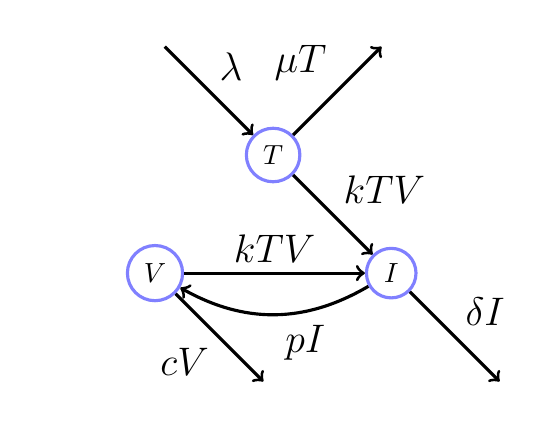
\begin{tikzpicture}[place/.style={circle,draw=blue!50,line width=0.4mm, fill=white},
   transition/.style={->,line width=0.4mm}, scale = 0.5]
\node[place] (t) at (0, 0) {$T$};

\node[place](i) at (3, -3) {$I$};

\node[place](v) at (-3, -3) {$V$};

\node[](vpathstart) at (-6, 0) {};

\node[](vpathend)at (0, -6) {};

\node[](tpathstart) at (-3, 3){};

\node[](tpathend) at (6, -6) {};

\node[](tpathend2) at (3, 3) {};

\node[](vpathend2) at (1.55, -1.3) {};

\path
	(tpathstart) edge[transition] node [auto]{{\Large $\lambda$}}(t)
	(t) edge[transition] node[auto] {\Large{$kTV$}}(i)
	(i) edge[transition] node [auto] {\Large{$\delta I$}} (tpathend)
%	(v) edge[transition] node [auto] {\Large{$pI$}} (i)
	(i) edge[transition, bend left=30] node [below right] {\Large{$pI$}} (v)
	(v) edge[transition] node [below left] {\Large{$cV$}} (vpathend)
	(t) edge[transition] node [auto] {\Large{$\mu T$}} (tpathend2)
	(v) edge[transition] node[auto] {\Large{$kTV$}}(i)
%	(v) edge[transition] (vpathend2)
;
	    

\end{tikzpicture}
\caption{Illustration of 3CM}
\label{tikz3CM}
\end{center}
\end{figure}
\begin{figure}
\begin{center}
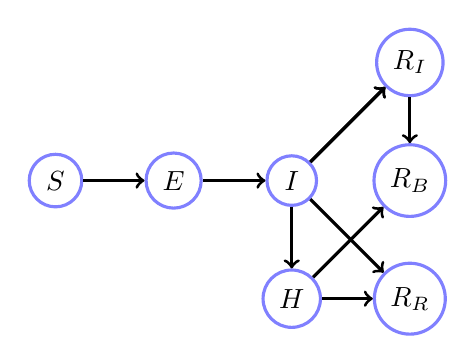
\begin{tikzpicture}[place/.style={circle,draw=blue!50,line width=0.4mm, fill=white},
   transition/.style={->,line width=0.4mm}, scale = 0.5]
\node[place] (s) at (-6, 0) {$S$};
\node[place] (e) at (-3, 0) {$E$};
\node[place] (i) at (0, 0) {$I$};
\node[place] (rb) at (3, 0) {$R_B$};
\node[place](ri) at (3, 3) {$R_I$};
\node[place](rr) at (3, -3) {$R_R$};
\node[place](h) at (0, -3) {$H$};

\path
    (s) edge[transition] node[auto]{} (e)
    (e) edge[transition] node[auto]{} (i)
    (i) edge[transition] node[auto]{} (ri)
    (ri) edge[transition] node[auto]{} (rb)
    (i) edge[transition] node[auto]{} (ri)
    (i) edge[transition] node[auto]{} (rr)
    (i) edge[transition] node[auto]{} (h)
    (h) edge[transition] node[auto]{} (rr)
    (h) edge[transition] node[auto]{} (rb)

;
	    

\end{tikzpicture}
\caption{Illustration of ebola model}
\label{tikz3CM}
\end{center}
\end{figure}
\end{document}
